\documentclass[12pt]{article}


\usepackage{fancyhdr}
\usepackage{extramarks}
\usepackage{amsthm}
\usepackage{amssymb}
\usepackage{subfigure}
\usepackage{amsmath}
\usepackage{amssymb}
\usepackage{bm}
\usepackage{amsfonts}
\usepackage{tikz}
\usepackage[plain]{algorithm}
\usepackage{algpseudocode}
\usepackage[colorlinks=true]{hyperref}
\usepackage[colorinlistoftodos,prependcaption,textsize=tiny]{todonotes}
\usepackage{scrextend}



%\setlength{\parskip}{\baselineskip}
%\setlength{\parindent}{0pt}

\usetikzlibrary{automata,positioning,fit}

%
% Basic Document Settings
%

\setlength{\parindent}{0cm}
\addtolength{\oddsidemargin}{-2cm}
\addtolength{\evensidemargin}{-2cm}
\setlength{\textwidth}{17.78cm}
\addtolength{\topmargin}{-2.25cm}
\setlength{\textheight}{23.24cm}
\addtolength{\parskip}{5mm}



\pagestyle{fancy}
%\lhead{\hmwkAuthorName}
\lhead{\hmwkClass\ (\hmwkClassInstructor) \#\hmwkNumber}
\rhead{\firstxmark}
\lfoot{\lastxmark}
\cfoot{\thepage}

\renewcommand\headrulewidth{0.4pt}
\renewcommand\footrulewidth{0.4pt}

\newcommand{\staritem}{
\addtocounter{enumi}{1}
\item[$\phantom{x}^{*}$\theenumi]}

\setlength\parindent{0pt}


%%%%% NEW MATH DEFINITIONS %%%%%

% Mark sections of captions for referring to divisions of figures
\newcommand{\figleft}{{\em (Left)}}
\newcommand{\figcenter}{{\em (Center)}}
\newcommand{\figright}{{\em (Right)}}
\newcommand{\figtop}{{\em (Top)}}
\newcommand{\figbottom}{{\em (Bottom)}}
\newcommand{\captiona}{{\em (a)}}
\newcommand{\captionb}{{\em (b)}}
\newcommand{\captionc}{{\em (c)}}
\newcommand{\captiond}{{\em (d)}}

% Highlight a newly defined term
\newcommand{\newterm}[1]{{\bf #1}}


% Figure reference, lower-case.
\def\figref#1{figure~\ref{#1}}
% Figure reference, capital. For start of sentence
\def\Figref#1{Figure~\ref{#1}}
\def\twofigref#1#2{figures \ref{#1} and \ref{#2}}
\def\quadfigref#1#2#3#4{figures \ref{#1}, \ref{#2}, \ref{#3} and \ref{#4}}
% Section reference, lower-case.
\def\secref#1{section~\ref{#1}}
% Section reference, capital.
\def\Secref#1{Section~\ref{#1}}
% Reference to two sections.
\def\twosecrefs#1#2{sections \ref{#1} and \ref{#2}}
% Reference to three sections.
\def\secrefs#1#2#3{sections \ref{#1}, \ref{#2} and \ref{#3}}
% Reference to an equation, lower-case.
\def\eqref#1{equation~\ref{#1}}
% Reference to an equation, upper case
\def\Eqref#1{Equation~\ref{#1}}
% A raw reference to an equation---avoid using if possible
\def\plaineqref#1{\ref{#1}}
% Reference to a chapter, lower-case.
\def\chapref#1{chapter~\ref{#1}}
% Reference to an equation, upper case.
\def\Chapref#1{Chapter~\ref{#1}}
% Reference to a range of chapters
\def\rangechapref#1#2{chapters\ref{#1}--\ref{#2}}
% Reference to an algorithm, lower-case.
\def\algref#1{algorithm~\ref{#1}}
% Reference to an algorithm, upper case.
\def\Algref#1{Algorithm~\ref{#1}}
\def\twoalgref#1#2{algorithms \ref{#1} and \ref{#2}}
\def\Twoalgref#1#2{Algorithms \ref{#1} and \ref{#2}}
% Reference to a part, lower case
\def\partref#1{part~\ref{#1}}
% Reference to a part, upper case
\def\Partref#1{Part~\ref{#1}}
\def\twopartref#1#2{parts \ref{#1} and \ref{#2}}

\def\ceil#1{\lceil #1 \rceil}
\def\floor#1{\lfloor #1 \rfloor}
\def\1{\bm{1}}
\newcommand{\train}{\mathcal{D}}
\newcommand{\valid}{\mathcal{D_{\mathrm{valid}}}}
\newcommand{\test}{\mathcal{D_{\mathrm{test}}}}

\def\eps{{\epsilon}}


% Random variables
\def\reta{{\textnormal{$\eta$}}}
\def\ra{{\textnormal{a}}}
\def\rb{{\textnormal{b}}}
\def\rc{{\textnormal{c}}}
\def\rd{{\textnormal{d}}}
\def\re{{\textnormal{e}}}
\def\rf{{\textnormal{f}}}
\def\rg{{\textnormal{g}}}
\def\rh{{\textnormal{h}}}
\def\ri{{\textnormal{i}}}
\def\rj{{\textnormal{j}}}
\def\rk{{\textnormal{k}}}
\def\rl{{\textnormal{l}}}
% rm is already a command, just don't name any random variables m
\def\rn{{\textnormal{n}}}
\def\ro{{\textnormal{o}}}
\def\rp{{\textnormal{p}}}
\def\rq{{\textnormal{q}}}
\def\rr{{\textnormal{r}}}
\def\rs{{\textnormal{s}}}
\def\rt{{\textnormal{t}}}
\def\ru{{\textnormal{u}}}
\def\rv{{\textnormal{v}}}
\def\rw{{\textnormal{w}}}
\def\rx{{\textnormal{x}}}
\def\ry{{\textnormal{y}}}
\def\rz{{\textnormal{z}}}

% Random vectors
\def\rvepsilon{{\mathbf{\epsilon}}}
\def\rvtheta{{\mathbf{\theta}}}
\def\rva{{\mathbf{a}}}
\def\rvb{{\mathbf{b}}}
\def\rvc{{\mathbf{c}}}
\def\rvd{{\mathbf{d}}}
\def\rve{{\mathbf{e}}}
\def\rvf{{\mathbf{f}}}
\def\rvg{{\mathbf{g}}}
\def\rvh{{\mathbf{h}}}
\def\rvu{{\mathbf{i}}}
\def\rvj{{\mathbf{j}}}
\def\rvk{{\mathbf{k}}}
\def\rvl{{\mathbf{l}}}
\def\rvm{{\mathbf{m}}}
\def\rvn{{\mathbf{n}}}
\def\rvo{{\mathbf{o}}}
\def\rvp{{\mathbf{p}}}
\def\rvq{{\mathbf{q}}}
\def\rvr{{\mathbf{r}}}
\def\rvs{{\mathbf{s}}}
\def\rvt{{\mathbf{t}}}
\def\rvu{{\mathbf{u}}}
\def\rvv{{\mathbf{v}}}
\def\rvw{{\mathbf{w}}}
\def\rvx{{\mathbf{x}}}
\def\rvy{{\mathbf{y}}}
\def\rvz{{\mathbf{z}}}

% Elements of random vectors
\def\erva{{\textnormal{a}}}
\def\ervb{{\textnormal{b}}}
\def\ervc{{\textnormal{c}}}
\def\ervd{{\textnormal{d}}}
\def\erve{{\textnormal{e}}}
\def\ervf{{\textnormal{f}}}
\def\ervg{{\textnormal{g}}}
\def\ervh{{\textnormal{h}}}
\def\ervi{{\textnormal{i}}}
\def\ervj{{\textnormal{j}}}
\def\ervk{{\textnormal{k}}}
\def\ervl{{\textnormal{l}}}
\def\ervm{{\textnormal{m}}}
\def\ervn{{\textnormal{n}}}
\def\ervo{{\textnormal{o}}}
\def\ervp{{\textnormal{p}}}
\def\ervq{{\textnormal{q}}}
\def\ervr{{\textnormal{r}}}
\def\ervs{{\textnormal{s}}}
\def\ervt{{\textnormal{t}}}
\def\ervu{{\textnormal{u}}}
\def\ervv{{\textnormal{v}}}
\def\ervw{{\textnormal{w}}}
\def\ervx{{\textnormal{x}}}
\def\ervy{{\textnormal{y}}}
\def\ervz{{\textnormal{z}}}

% Random matrices
\def\rmA{{\mathbf{A}}}
\def\rmB{{\mathbf{B}}}
\def\rmC{{\mathbf{C}}}
\def\rmD{{\mathbf{D}}}
\def\rmE{{\mathbf{E}}}
\def\rmF{{\mathbf{F}}}
\def\rmG{{\mathbf{G}}}
\def\rmH{{\mathbf{H}}}
\def\rmI{{\mathbf{I}}}
\def\rmJ{{\mathbf{J}}}
\def\rmK{{\mathbf{K}}}
\def\rmL{{\mathbf{L}}}
\def\rmM{{\mathbf{M}}}
\def\rmN{{\mathbf{N}}}
\def\rmO{{\mathbf{O}}}
\def\rmP{{\mathbf{P}}}
\def\rmQ{{\mathbf{Q}}}
\def\rmR{{\mathbf{R}}}
\def\rmS{{\mathbf{S}}}
\def\rmT{{\mathbf{T}}}
\def\rmU{{\mathbf{U}}}
\def\rmV{{\mathbf{V}}}
\def\rmW{{\mathbf{W}}}
\def\rmX{{\mathbf{X}}}
\def\rmY{{\mathbf{Y}}}
\def\rmZ{{\mathbf{Z}}}

% Elements of random matrices
\def\ermA{{\textnormal{A}}}
\def\ermB{{\textnormal{B}}}
\def\ermC{{\textnormal{C}}}
\def\ermD{{\textnormal{D}}}
\def\ermE{{\textnormal{E}}}
\def\ermF{{\textnormal{F}}}
\def\ermG{{\textnormal{G}}}
\def\ermH{{\textnormal{H}}}
\def\ermI{{\textnormal{I}}}
\def\ermJ{{\textnormal{J}}}
\def\ermK{{\textnormal{K}}}
\def\ermL{{\textnormal{L}}}
\def\ermM{{\textnormal{M}}}
\def\ermN{{\textnormal{N}}}
\def\ermO{{\textnormal{O}}}
\def\ermP{{\textnormal{P}}}
\def\ermQ{{\textnormal{Q}}}
\def\ermR{{\textnormal{R}}}
\def\ermS{{\textnormal{S}}}
\def\ermT{{\textnormal{T}}}
\def\ermU{{\textnormal{U}}}
\def\ermV{{\textnormal{V}}}
\def\ermW{{\textnormal{W}}}
\def\ermX{{\textnormal{X}}}
\def\ermY{{\textnormal{Y}}}
\def\ermZ{{\textnormal{Z}}}

% Vectors
\def\vzero{{\bm{0}}}
\def\vone{{\bm{1}}}
\def\vmu{{\bm{\mu}}}
\def\vtheta{{\bm{\theta}}}
\def\va{{\bm{a}}}
\def\vb{{\bm{b}}}
\def\vc{{\bm{c}}}
\def\vd{{\bm{d}}}
\def\ve{{\bm{e}}}
\def\vf{{\bm{f}}}
\def\vg{{\bm{g}}}
\def\vh{{\bm{h}}}
\def\vi{{\bm{i}}}
\def\vj{{\bm{j}}}
\def\vk{{\bm{k}}}
\def\vl{{\bm{l}}}
\def\vm{{\bm{m}}}
\def\vn{{\bm{n}}}
\def\vo{{\bm{o}}}
\def\vp{{\bm{p}}}
\def\vq{{\bm{q}}}
\def\vr{{\bm{r}}}
\def\vs{{\bm{s}}}
\def\vt{{\bm{t}}}
\def\vu{{\bm{u}}}
\def\vv{{\bm{v}}}
\def\vw{{\bm{w}}}
\def\vx{{\bm{x}}}
\def\vy{{\bm{y}}}
\def\vz{{\bm{z}}}

% Elements of vectors
\def\evalpha{{\alpha}}
\def\evbeta{{\beta}}
\def\evepsilon{{\epsilon}}
\def\evlambda{{\lambda}}
\def\evomega{{\omega}}
\def\evmu{{\mu}}
\def\evpsi{{\psi}}
\def\evsigma{{\sigma}}
\def\evtheta{{\theta}}
\def\eva{{a}}
\def\evb{{b}}
\def\evc{{c}}
\def\evd{{d}}
\def\eve{{e}}
\def\evf{{f}}
\def\evg{{g}}
\def\evh{{h}}
\def\evi{{i}}
\def\evj{{j}}
\def\evk{{k}}
\def\evl{{l}}
\def\evm{{m}}
\def\evn{{n}}
\def\evo{{o}}
\def\evp{{p}}
\def\evq{{q}}
\def\evr{{r}}
\def\evs{{s}}
\def\evt{{t}}
\def\evu{{u}}
\def\evv{{v}}
\def\evw{{w}}
\def\evx{{x}}
\def\evy{{y}}
\def\evz{{z}}

% Matrix
\def\mA{{\bm{A}}}
\def\mB{{\bm{B}}}
\def\mC{{\bm{C}}}
\def\mD{{\bm{D}}}
\def\mE{{\bm{E}}}
\def\mF{{\bm{F}}}
\def\mG{{\bm{G}}}
\def\mH{{\bm{\text{\textbf{H}}}}}
\def\mI{{\bm{I}}}
\def\mJ{{\bm{J}}}
\def\mK{{\bm{K}}}
\def\mL{{\bm{L}}}
\def\mM{{\bm{M}}}
\def\mN{{\bm{N}}}
\def\mO{{\bm{O}}}
\def\mP{{\bm{P}}}
\def\mQ{{\bm{Q}}}
\def\mR{{\bm{R}}}
\def\mS{{\bm{S}}}
\def\mT{{\bm{T}}}
\def\mU{{\bm{U}}}
\def\mV{{\bm{V}}}
\def\mW{{\bm{W}}}
\def\mX{{\bm{X}}}
\def\mY{{\bm{Y}}}
\def\mZ{{\bm{Z}}}
\def\mBeta{{\bm{\beta}}}
\def\mPhi{{\bm{\Phi}}}
\def\mLambda{{\bm{\Lambda}}}
\def\mSigma{{\bm{\Sigma}}}

% Tensor
\DeclareMathAlphabet{\mathsfit}{\encodingdefault}{\sfdefault}{m}{sl}
\SetMathAlphabet{\mathsfit}{bold}{\encodingdefault}{\sfdefault}{bx}{n}
\newcommand{\tens}[1]{\bm{\mathsfit{#1}}}
\def\tA{{\tens{A}}}
\def\tB{{\tens{B}}}
\def\tC{{\tens{C}}}
\def\tD{{\tens{D}}}
\def\tE{{\tens{E}}}
\def\tF{{\tens{F}}}
\def\tG{{\tens{G}}}
\def\tH{{\tens{H}}}
\def\tI{{\tens{I}}}
\def\tJ{{\tens{J}}}
\def\tK{{\tens{K}}}
\def\tL{{\tens{L}}}
\def\tM{{\tens{M}}}
\def\tN{{\tens{N}}}
\def\tO{{\tens{O}}}
\def\tP{{\tens{P}}}
\def\tQ{{\tens{Q}}}
\def\tR{{\tens{R}}}
\def\tS{{\tens{S}}}
\def\tT{{\tens{T}}}
\def\tU{{\tens{U}}}
\def\tV{{\tens{V}}}
\def\tW{{\tens{W}}}
\def\tX{{\tens{X}}}
\def\tY{{\tens{Y}}}
\def\tZ{{\tens{Z}}}


% Graph
\def\gA{{\mathcal{A}}}
\def\gB{{\mathcal{B}}}
\def\gC{{\mathcal{C}}}
\def\gD{{\mathcal{D}}}
\def\gE{{\mathcal{E}}}
\def\gF{{\mathcal{F}}}
\def\gG{{\mathcal{G}}}
\def\gH{{\mathcal{H}}}
\def\gI{{\mathcal{I}}}
\def\gJ{{\mathcal{J}}}
\def\gK{{\mathcal{K}}}
\def\gL{{\mathcal{L}}}
\def\gM{{\mathcal{M}}}
\def\gN{{\mathcal{N}}}
\def\gO{{\mathcal{O}}}
\def\gP{{\mathcal{P}}}
\def\gQ{{\mathcal{Q}}}
\def\gR{{\mathcal{R}}}
\def\gS{{\mathcal{S}}}
\def\gT{{\mathcal{T}}}
\def\gU{{\mathcal{U}}}
\def\gV{{\mathcal{V}}}
\def\gW{{\mathcal{W}}}
\def\gX{{\mathcal{X}}}
\def\gY{{\mathcal{Y}}}
\def\gZ{{\mathcal{Z}}}

% Sets
\def\sA{{\mathbb{A}}}
\def\sB{{\mathbb{B}}}
\def\sC{{\mathbb{C}}}
\def\sD{{\mathbb{D}}}
% Don't use a set called E, because this would be the same as our symbol
% for expectation.
\def\sF{{\mathbb{F}}}
\def\sG{{\mathbb{G}}}
\def\sH{{\mathbb{H}}}
\def\sI{{\mathbb{I}}}
\def\sJ{{\mathbb{J}}}
\def\sK{{\mathbb{K}}}
\def\sL{{\mathbb{L}}}
\def\sM{{\mathbb{M}}}
\def\sN{{\mathbb{N}}}
\def\sO{{\mathbb{O}}}
\def\sP{{\mathbb{P}}}
\def\sQ{{\mathbb{Q}}}
\def\sR{{\mathbb{R}}}
\def\sS{{\mathbb{S}}}
\def\sT{{\mathbb{T}}}
\def\sU{{\mathbb{U}}}
\def\sV{{\mathbb{V}}}
\def\sW{{\mathbb{W}}}
\def\sX{{\mathbb{X}}}
\def\sY{{\mathbb{Y}}}
\def\sZ{{\mathbb{Z}}}

% Entries of a matrix
\def\emLambda{{\Lambda}}
\def\emA{{A}}
\def\emB{{B}}
\def\emC{{C}}
\def\emD{{D}}
\def\emE{{E}}
\def\emF{{F}}
\def\emG{{G}}
\def\emH{{H}}
\def\emI{{I}}
\def\emJ{{J}}
\def\emK{{K}}
\def\emL{{L}}
\def\emM{{M}}
\def\emN{{N}}
\def\emO{{O}}
\def\emP{{P}}
\def\emQ{{Q}}
\def\emR{{R}}
\def\emS{{S}}
\def\emT{{T}}
\def\emU{{U}}
\def\emV{{V}}
\def\emW{{W}}
\def\emX{{X}}
\def\emY{{Y}}
\def\emZ{{Z}}
\def\emSigma{{\Sigma}}

% entries of a tensor
% Same font as tensor, without \bm wrapper
\newcommand{\etens}[1]{\mathsfit{#1}}
\def\etLambda{{\etens{\Lambda}}}
\def\etA{{\etens{A}}}
\def\etB{{\etens{B}}}
\def\etC{{\etens{C}}}
\def\etD{{\etens{D}}}
\def\etE{{\etens{E}}}
\def\etF{{\etens{F}}}
\def\etG{{\etens{G}}}
\def\etH{{\etens{H}}}
\def\etI{{\etens{I}}}
\def\etJ{{\etens{J}}}
\def\etK{{\etens{K}}}
\def\etL{{\etens{L}}}
\def\etM{{\etens{M}}}
\def\etN{{\etens{N}}}
\def\etO{{\etens{O}}}
\def\etP{{\etens{P}}}
\def\etQ{{\etens{Q}}}
\def\etR{{\etens{R}}}
\def\etS{{\etens{S}}}
\def\etT{{\etens{T}}}
\def\etU{{\etens{U}}}
\def\etV{{\etens{V}}}
\def\etW{{\etens{W}}}
\def\etX{{\etens{X}}}
\def\etY{{\etens{Y}}}
\def\etZ{{\etens{Z}}}

% The true underlying data generating distribution
\newcommand{\pdata}{p_{\rm{data}}}
% The empirical distribution defined by the training set
\newcommand{\ptrain}{\hat{p}_{\rm{data}}}
\newcommand{\Ptrain}{\hat{P}_{\rm{data}}}
% The model distribution
\newcommand{\pmodel}{p_{\rm{model}}}
\newcommand{\Pmodel}{P_{\rm{model}}}
\newcommand{\ptildemodel}{\tilde{p}_{\rm{model}}}
% Stochastic autoencoder distributions
\newcommand{\pencode}{p_{\rm{encoder}}}
\newcommand{\pdecode}{p_{\rm{decoder}}}
\newcommand{\precons}{p_{\rm{reconstruct}}}

\newcommand{\laplace}{\mathrm{Laplace}} % Laplace distribution

\newcommand{\E}{\mathbb{E}}
\newcommand{\Ls}{\mathcal{L}}
\newcommand{\R}{\mathbb{R}}
\newcommand{\emp}{\tilde{p}}
\newcommand{\lr}{\alpha}
\newcommand{\reg}{\lambda}
\newcommand{\rect}{\mathrm{rectifier}}
\newcommand{\softmax}{\mathrm{softmax}}
\newcommand{\sigmoid}{\sigma}
\newcommand{\softplus}{\zeta}
\newcommand{\KL}{D_{\mathrm{KL}}}
\newcommand{\Var}{\mathrm{Var}}
\newcommand{\standarderror}{\mathrm{SE}}
\newcommand{\Cov}{\mathrm{Cov}}
% Wolfram Mathworld says $L^2$ is for function spaces and $\ell^2$ is for vectors
% But then they seem to use $L^2$ for vectors throughout the site, and so does
% wikipedia.
\newcommand{\normlzero}{L^0}
\newcommand{\normlone}{L^1}
\newcommand{\normltwo}{L^2}
\newcommand{\normlp}{L^p}
\newcommand{\normmax}{L^\infty}

\newcommand{\parents}{Pa} % See usage in notation.tex. Chosen to match Daphne's book.

\DeclareMathOperator*{\argmax}{arg\,max}
\DeclareMathOperator*{\argmin}{arg\,min}

\DeclareMathOperator{\sign}{sign}
\DeclareMathOperator{\Tr}{Tr}
\let\ab\allowbreak


%%% new
\newcommand{\diag}{\mathop{\mathrm{diag}}\nolimits}
\usepackage{cancel}
\newcommand{\ttt}[1]{\texttt{#1}}

%
% Create Problem Sections
%

\newcommand{\enterProblemHeader}[1]{
    \nobreak\extramarks{}{Problem \arabic{#1} continued on next page\ldots}\nobreak{}
    \nobreak\extramarks{Problem \arabic{#1} (continued)}{Problem \arabic{#1} continued on next page\ldots}\nobreak{}
}

\newcommand{\exitProblemHeader}[1]{
    \nobreak\extramarks{Problem \arabic{#1} (continued)}{Problem \arabic{#1} continued on next page\ldots}\nobreak{}
    \stepcounter{#1}
    \nobreak\extramarks{Problem \arabic{#1}}{}\nobreak{}
}

\setcounter{secnumdepth}{0}
\newcounter{partCounter}
\newcounter{homeworkProblemCounter}
\setcounter{homeworkProblemCounter}{1}
\nobreak\extramarks{Problem \arabic{homeworkProblemCounter}}{}\nobreak{}

%
% Homework Problem Environment
%
% This environment takes an optional argument. When given, it will adjust the
% problem counter. This is useful for when the problems given for your
% assignment aren't sequential. See the last 3 problems of this template for an
% example.
%
\newenvironment{homeworkProblem}[1][-1]{
    \ifnum#1>0
        \setcounter{homeworkProblemCounter}{#1}
    \fi
    \section{Problem \arabic{homeworkProblemCounter}}
    \setcounter{partCounter}{1}
    \enterProblemHeader{homeworkProblemCounter}
}{
    \exitProblemHeader{homeworkProblemCounter}
}

%
% Homework Details
%   - Title
%   - Due date
%   - Class
%   - Section/Time
%   - Instructor
%   - Author
%

\newcommand{\hmwkTitle}{Homework \hmwkNumber}
\newcommand{\hmwkNumber}{2}
\newcommand{\hmwkDueDate}{TODO}
\newcommand{\hmwkClass}{IFT6135H18 - Representation Learning}
\newcommand{\hmwkClassInstructor}{Aaron Courville}


%
% Title Page
%

\title{
    \vspace{0in}
    \textmd{\textbf{\hmwkClass}}\\
    \hmwkTitle \ - Programming Part\\
    \normalsize\vspace{0.1in}\small{Due\ on\ \hmwkDueDate}\\
    \vspace{0.1in}\large{Instructor: \textit{\hmwkClassInstructor\\}} 
    \vspace{0in}
}

%\author{\hmwkAuthorName}
%\date{}

\renewcommand{\part}[1]{\textbf{\large Part \Alph{partCounter}}\stepcounter{partCounter}\\}



%
% Various Helper Commands
%

% Useful for algorithms
\newcommand{\alg}[1]{\textsc{\bfseries \footnotesize #1}}
% For derivatives
\newcommand{\deriv}[1]{\frac{\mathrm{d}}{\mathrm{d}x} (#1)}
% Integral dx
\newcommand{\dx}{\mathrm{d}x}
% Alias for the Solution section header
\newcommand{\solution}{\textbf{\large Solution}}
% Probability commands: Expectation, Variance, Covariance, Bias

\newcommand{\Bias}{\mathrm{Bias}}
\newcommand{\N}{\mathcal{N}}



\begin{document}


\fancyhead{}
\fancyfoot{}

\fancyhead[L]{
  \begin{tabular}[b]{l}
    IFT6135-A2023  \\
    Prof: Aishwarya Agrawal \\
  \end{tabular}
}
\fancyhead[R]{
  \begin{tabular}[b]{r}
    Assignment 2, Programming Part   \\
    RNN, Optimization, Regularization and Normalization \\
  \end{tabular}
}
\fancyfoot[C]{- Do not distribute -}

{\bf Due Date: Monday, 14th November, 11pm ET}

\vspace{-0.5cm}
\uline{The use of AI tools like Chat-GPT to find answers or parts of answers for any question in this assignment is not allowed. However, you can use these tools to improve the quality of your writing, like fixing grammar or making it more understandable. If you do use these tools, you must clearly explain how you used them and which questions or parts of questions you applied them to. Failing to do so or using these tools to find answers or parts of answers may result in your work being completely rejected, which means you'll receive a score of 0 for the entire practical section.}


\renewcommand{\labelitemi}{\textbullet}

\begin{itemize}
\item \emph{This assignment is intensive, start well ahead of time!}
\item \emph{For all questions, show your work.}
\item \emph{The practical part has been provided to you as a zip file. To utilize the GPU capabilities of Google Colab, please put the zip file in your google drive and open it within Google Colab. Then, follow the instructions outlined in the \texttt{main.py} file to ensure compatibility with Google Colab. You must fill in your answers in the notebook and export the notebook as two Python file named \texttt{lstm\_solution.py} and \texttt{gpt1\_solution.py} (File$\xrightarrow{}$Download$\xrightarrow{}$Download .py) and submit both via Gradescope for autograding.}
\item \emph{You must also submit your report (PDF) on Gradescope. Your report must contain answers to Problem 3. You do not need to submit code for these questions, just the report will suffice.}
\item \emph{TAs for this assignment are \textbf{Sophie Xhonneux and Sahar Dastani}.}
\end{itemize}
\vspace{0.2cm}


\setlength{\parindent}{1cm}
\paragraph{Assignment File:} Link \href{https://drive.google.com/file/d/1E10mBJbB1pNFDgUJgPOrSXjW0AqQdS4B/view?usp=sharing}{click here}

\paragraph{Gradescope:}

Please submit \textbf{two} files: 
\begin{itemize}
    \item \texttt{lstm\_solution.py}
    \item \texttt{gpt1\_solution.py}
\end{itemize}

\paragraph{Summary:}

{$ $}

\noindent In this assignment, you will perform \textbf{sequential language modeling} on the \href{https://blog.einstein.ai/the-wikitext-long-term-dependency-language-modeling-dataset/}{Wikitext-2} dataset. The dataset contains sequences of \emph{tokens} (i.e., words or subwords) extracted from contiguous sentences. Each unique token is denoted by an integer in the range $[1, N]$, where $N$ is the number of all unique tokens ($N$ is also often referred to as the \emph{vocabulary size}). For this assignment, we use a vocabulary of size $N = 40,478$, as originally defined for OpenAI's GPT. Sequential language models do \emph{next-word prediction}: they predict tokens in a sequence one at a time, with each prediction based on all the previous elements of the sequence. A trained sequential language model can then be used to generate new sequences of text, by making each prediction conditioned on the past \emph{predictions}.

\noindent In this assignment, you will implement a sequential language model (an \textbf{LSTM}), and a masked language model (\textbf{Transformer} inspired by OpenAI GPT). In problem 1, you will use built-in PyTorch modules to implement an LSTM. In problem 2, you will implement various building blocks of a transformer, including \textbf{LayerNorm} (layer normalization) and the \textbf{Attention} mechanism.

\paragraph{The Wikitext-2 dataset} comprises 2 million words extracted from the set of verified ``Good'' and ``Featured'' articles on Wikipedia. See this \href{https://blog.einstein.ai/the-wikitext-long-term-dependency-language-modeling-dataset/}{blog post} for details about the Wikitext dataset and sample data. The dataset you get with the assignment has already been preprocessed using OpenAI's GPT vocabulary, and each file is a compressed numpy array containing two arrays: \texttt{tokens} containing a flattened list of (integer) tokens, and \texttt{sizes} containing the size of each document.

\noindent You are provided a PyTorch dataset class (\href{https://pytorch.org/docs/stable/data.html#torch.utils.data.Dataset}{\texttt{torch.utils.data.Dataset}}) named \texttt{Wikitext2} in the \texttt{utils} folder. This class loads the Wikitext-2 dataset and generates fixed-length sequences from it. Throughout this assignment, \textbf{all sequences will have length 256}, and we will use zero-padding to pad shorter sequences. Each sample from the dataset is a dictionary containing 3 keys: \texttt{source} (the input sequence), \texttt{target} (the target sequence, which is just the input sequence shifted one position to the left)), and \texttt{mask} (a binary vector of the same shape as the input indicating whether the token is valid ($1$), or is just a zero-padding to get the sequence length to $256$). For example (the sequences have been shortened for presentation):
\begin{table}[H]
    \centering
    \begin{tabular}{lccccccccl}
        \texttt{source} & 304 & 4731 & 8406 & 614 & 0 & 0 & 0 & $\ldots$ & \hspace{3em} \texttt{torch.LongTensor} \\
        \texttt{target} & 4731 & 8406 & 614 & 304 & 0 & 0 & 0 & $\ldots$ & \hspace{3em} \texttt{torch.LongTensor} \\
        \texttt{mask} & 1 & 1 & 1 & 1 & 0 & 0 & 0 & $\ldots$ & \hspace{3em} \texttt{torch.FloatTensor}
    \end{tabular}
    \label{tab:wikitext2-dataset}
\end{table}
\noindent In practice though, you will work with mini-batches of data, each with batchsize \texttt{B} elements. You can wrap this dataset object into a \href{https://pytorch.org/docs/stable/data.html#torch.utils.data.DataLoader}{\texttt{torch.utils.data.DataLoader}}, which will return a dictionary with keys \texttt{source}, \texttt{target}, and \texttt{mask}, each of shape \texttt{(B, 256)}.
% When fed into a PyTorch dataloader, you will then get a batch of data as a dictionary containing the same keys, with all 3 tensors of size \texttt{(batch\_size, 256)}.

\paragraph{Tests}: For you to quickly verify that all the functions you implemented have  valid input-output signatures (e.g. tensor types and shapes), we have provided public tests that will check if your output tensors have the correct shape, given random input data. Check the comments (docstrings) in each function to see what input/output shapes are expected. We recommend you to run these tests locally while completing the functions using the following command (to run inside your assignment folder)\\[0.5em]
\begin{minipage}{\linewidth}
\centering
\texttt{python -m unittest}
\end{minipage}\\[0.5em]
For students using Google Colab to complete their assignments, a cell with this command is available in the \texttt{main.ipynb} notebook. Note that these tests are not testing if the values returned by the functions are valid (only if the tensor shapes are correct), and will not be graded. You will be graded on a separate set of tests in Gradescope.

\noindent If the tests on Gradescope fail, as a rule of thumb $x$ corresponds to the value in your assignment (e.g. the value returned by your function), and $y$ is the expected value.

\paragraph{Emebeddings \& parameter sharing} In both the LSTM and the Transformer, the embedding layer is among the layers that contain the most parameters. Indeed, it consists of a matrix of size \texttt{(vocabulary\_size, embedding\_size)} (note that here \texttt{vocabulary\_size} is equal to $N + 1$, to account for zero-padding), which represents about 31M parameters. Similarly, in both models, we also have a classifier of about the same size (i.e. the output has size \texttt{vocabulary\_size} as well, to represent the probability of the next word). In order to speed up training, and for simplification in this assignment, we make two assumptions for both models:
\begin{itemize}
    \item Following the architecture from OpenAI's GPT, the weights of the classifier layer and the embedding layer will be shared.
    \item You will use pretrained embeddings from OpenAI's GPT (they are provided in the \texttt{run\_exp.py} script, described in Problem 3), which will remain frozen over the course of training.
\end{itemize}

\paragraph{Coding instructions} You will be required to use PyTorch to complete all questions. Moreover, this assignment \textbf{requires running the models on GPU} (otherwise it will take an incredibly long time); if you don't have access to your own resources (e.g. your own machine, a cluster), please use Google Colab (the notebook \texttt{main.ipynb} is here to help you). For some questions, you will be asked to not use certain functions in PyTorch and implement these yourself using primitive functions from \texttt{torch}; in that case, the functions in question are explicitly disabled in the tests on Gradescope.

\setlength{\parindent}{0cm}

\begin{homeworkProblem}

%%%%%%%%%%%%%%%%%%%%%%%%%%%%%%%%%%%%%%%%%
%%%%%%%%%%%%%%%%%%%%%%%%%%%%%%%%%%%%%%%%%
\paragraph{Implementing an LSTM (9pts)} In this problem, you will be using PyTorch's built-in modules in order to implement an LSTM. The architecture you will be asked to implement is the following:\\[1em]
\begin{minipage}{\linewidth}
\centering
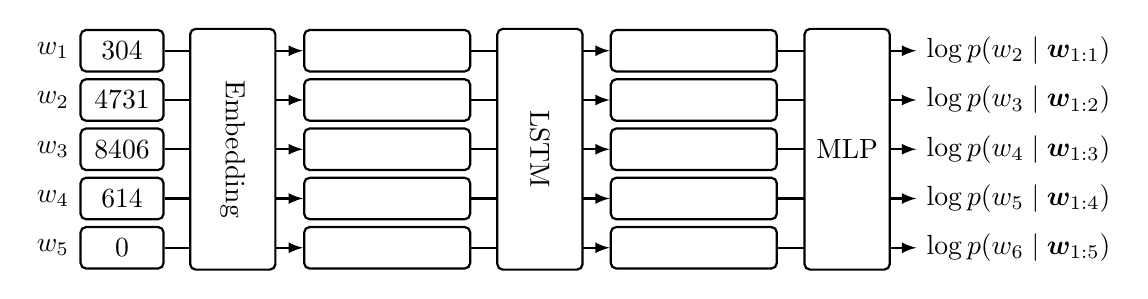
\begin{tikzpicture}[every node/.style={draw, thick, rounded corners=2pt, minimum height=1.5em}, token/.style={minimum width=3em}, vector/.style={minimum width=6em}]
    \node[token, label={180:$w_{1}$}] (in1) at (0, 0) {$304$};
    \node[token, below=2pt of in1, label={180:$w_{2}$}] (in2) {$4731$};
    \node[token, below=2pt of in2, label={180:$w_{3}$}] (in3) {$8406$};
    \node[token, below=2pt of in3, label={180:$w_{4}$}] (in4) {$614$};
    \node[token, below=2pt of in4, label={180:$w_{5}$}] (in5) {$0$};

    \foreach \i [evaluate=\i as \ip using {int(\i+1)}] in {1,...,5} {
        \node[vector, right=5em of in\i] (embed\i) {};
        \draw[-latex, thick] (in\i) -- (embed\i);
        \node[vector, right=5em of embed\i] (lstm\i) {};
        \draw[-latex, thick] (embed\i) -- (lstm\i);
        \node[vector, draw=none, right=5em of lstm\i] (logproba\i) {$\log p(w_{\ip} \mid \vw_{1:\i})$};
        \draw[-latex, thick] (lstm\i) -- (logproba\i);
    }
    
    \node[fit=(in1)(in2)(in3)(in4)(in5), inner sep=0pt, xshift=4em, fill=white] (embed_layer) {};
    \node[draw=none, inner sep=0pt, rotate=-90] at (embed_layer.center) {Embedding};
    
    \node[fit=(in1)(in2)(in3)(in4)(in5), inner sep=0pt, xshift=15.1em, fill=white] (lstm_layer) {};
    \node[draw=none, inner sep=0pt, rotate=-90] at (lstm_layer.center) {LSTM};
    
    \node[fit=(in1)(in2)(in3)(in4)(in5), inner sep=0pt, xshift=26.2em, fill=white] (lstm_layer) {};
    \node[draw=none, inner sep=0pt] at (lstm_layer.center) {MLP};
\end{tikzpicture}
\end{minipage}

\noindent In the file \texttt{lstm\_solution.py}, you are given an \texttt{LSTM} class containing all the blocks necessary to create this model. In particular, \texttt{self.embedding} is a \href{https://pytorch.org/docs/1.7.1/generated/torch.nn.Embedding.html}{\texttt{nn.Embedding}} module that converts sequences of token indices into embeddings, \texttt{self.lstm} is a \href{https://pytorch.org/docs/1.7.1/generated/torch.nn.LSTM.html}{\texttt{nn.LSTM}} module that runs an LSTM over a sequence of vectors, and \texttt{self.classifier} is a 2-layer MLP responsible for classification.

\begin{enumerate}
    \item Using the different modules described above, complete the \texttt{forward()} function. This function must return the log-probabilities (not the logits) of the next words in the sequence, as well as the final hidden state of the LSTM.
    
    \item Complete the \texttt{loss()} function, that returns the mean negative log-likelihood of the entire sequences in the minibatch (and also averaged over the mini-batch dimension). More precisely, for a single sequence in the mini-batch
    \begin{equation*}
        \mathcal{L}(\vtheta;\vw_{1:T+1}) = -\frac{1}{T}\sum_{t=1}^{T}\sum_{i=0}^{N}\log p(\widetilde{w}_{t+1} = i\mid \vw_{1:t};\vtheta)\vone(i = w_{t+1}),
    \end{equation*}
    where $\widetilde{w}$ are the predictions made by the model, and $\vone(i = w_{t+1})$ is the indicator function which equals $1$ if $i = w_{t+1}$, and $0$ otherwise. Note that here $T$ might be smaller than 256 (called \texttt{sequence\_length} in the code), because the sequence might be zero-padded; you may use \texttt{mask} for this. The \texttt{loss} function directly takes the log-probabilities as input (e.g. returned by the \texttt{forward} function).
\end{enumerate}

\end{homeworkProblem}
\begin{homeworkProblem}

%%%%%%%%%%%%%%%%%%%%%%%%%%%%%%%%%%%%%%%%%
%%%%%%%%%%%%%%%%%%%%%%%%%%%%%%%%%%%%%%%%%
\paragraph{Implementing a GPT (Generative-Pretrained Transformer)  (27pts)}
While typical RNNs ``remember'' past information by taking their previous hidden state as input at each step, recent years have seen a profusion of methodologies for making use of past information in different ways.
The transformer\footnote{See \url{https://arxiv.org/abs/1706.03762} for more details.} is one such fairly new architecture which uses several self-attention networks (``heads'') in parallel, among other architectural specifics.
Implementing a transformer is a fairly involved process -- so we provide most of the boilerplate code and your task is only to implement the multi-head scaled dot-product attention mechanism, as well as the layernorm operation.

\textbf{Implementing Layer Normalization (5pts)}: You will first implement the layer normalization (LayerNorm) technique that we have seen in class. For this assignment, \textbf{you are not allowed} to use the PyTorch \href{https://pytorch.org/docs/1.7.1/generated/torch.nn.LayerNorm.html#torch.nn.LayerNorm}{\texttt{nn.LayerNorm}} module (nor any function calling \texttt{torch.layer\_norm}).

As defined in the \href{https://arxiv.org/abs/1607.06450}{layer normalization paper}, the layernorm operation over a minibatch of inputs $x$ is defined as
\begin{equation*}
    \textnormal{layernorm}(x) = \frac{x - \E[x]}{\sqrt{\textnormal{Var}[x] + \epsilon}} * \texttt{weight} + \texttt{bias}
\end{equation*}
where $\E[x]$ denotes the expectation over $x$, $\textnormal{Var}[x]$ denotes the variance of $x$, both of which are only taken over the last dimension of the tensor $x$ here. \texttt{weight} and \texttt{bias} are learnable affine parameters.

\begin{enumerate}
    \item In the file \texttt{gpt1\_solution\_template.py}, implement the \texttt{forward()} function of the \texttt{LayerNorm} class. Pay extra attention to the lecture slides on the exact details of how $\E[x]$ and $\textnormal{Var}[x]$ are computed. In particular, PyTorch's function \href{https://pytorch.org/docs/1.7.1/generated/torch.var.html}{\texttt{torch.var}} uses an unbiased estimate of the variance by default, defined as the formula on the left-hand side
    \begin{align*}
        \overline{\Var}(X)_{\mathrm{unbiased}} &= \frac{1}{n-1}\sum_{i=1}^{n}(X_{i} - \overline{X})^{2} & \overline{\Var}(X)_{\mathrm{biased}} &= \frac{1}{n}\sum_{i=1}^{n}(X_{i} - \overline{X})^{2}
    \end{align*}
    whereas LayerNorm uses the biased estimate on the right-hand size (where $\overline{X}$ here is the mean estimate). Please refer to the docstrings of this function for more information on input/output signatures. 
\end{enumerate}

\textbf{Implementing the attention mechanism (17pts)}: You will now implement the core module of the transformer architecture -- the multi-head attention mechanism. Assuming there are $m$ attention heads, the attention vector for the head at index $i$ is given by:
% The attention vector for $m$ heads indexed by $i$ is calculated as follows: 
\begin{align*}
[\vq_{1}, \ldots, \vq_{m}] &= \mQ\mW_{Q} + \vb_{Q} \qquad [\vk_{1}, \ldots, \vk_{m}] = \mK\mW_{K} + \vb_{K} \qquad [\vv_{1}, \ldots, \vv_{m}] = \mV\mW_{V} + \vb_{V}\\
\mA_{i} &=\text{softmax}\left(\frac{\vq_{i}\vk_{i}^{\top}}{\sqrt{d}} \right)\\
\vh_{i} &= \mA_{i}\vv_{i} \\
A(\mQ, \mK, \mV) &= \text{concat}(\vh_{1}, \ldots, \vh_{m})\mW_{O} + \vb_{O}
\end{align*}
Here $\mQ, \mK, \mV$ are queries, keys, and values respectively, where all the heads have been concatenated into a single vector (e.g. here $\mK \in \sR^{T\times m d}$, where $d$ is the dimension of a single key vector, and $T$ the length of the sequence). $\mW_{Q}, \mW_{K}, \mW_{V}$ are the corresponding projection matrices (with biases $\vb$), and $\mW_O$ is the output projection (with bias $\vb_{O}$). $\mQ, \mK,$ and $\mV$ are determined by the output of the previous layer in the main network.
$\mA_i$ are the attention values, which specify which elements of the input sequence each attention head attends to. We recommend you to check \href{https://jalammar.github.io/illustrated-gpt2/}{this tutorial} for implementation details of GPT. In this question, \textbf{you are not allowed} to use the module \href{https://pytorch.org/docs/1.7.1/generated/torch.nn.MultiheadAttention.html}{\texttt{nn.MultiheadAttention}} (or any function calling \texttt{torch.nn.functional.multi\_head\_attention\_forward}). Please refer to the docstrings of each function for a precise description of what each function is expected to do, and the expected input/output tensors and their shapes.

\begin{enumerate}
    \setcounter{enumi}{1}
    \item The equations above require many vector manipulations in order to split and combine head vectors together. For example, the concatenated queries $\mQ$ are split into $m$ vectors $[\vq_{1}, \ldots, \vq_{m}]$ (one for each head) after an affine projection by $\mW_{Q}$, and the $h_{i}$'s are then concatenated back for the affine projection with $\mW_{O}$. In the class \texttt{MultiHeadedAttention}, implement the utility functions \texttt{split\_heads()} and \texttt{merge\_heads()} to do both of these operations, as well as a transposition for convenience later. For example, for the 1st sequence in the mini-batch:\\[0.5em]
    \begin{minipage}{\linewidth}
    \centering
    \begin{tabular}{lcl}
        \texttt{y = split\_heads(x)} & $\rightarrow$ & \texttt{y[0, 1, 2, 3] = x[0, 2, num\_heads * 1 + 3]}\\
        \texttt{x = merge\_heads(y)} & $\rightarrow$ & \texttt{x[0, 1, num\_heads * 2 + 3] = y[0, 2, 1, 3]}
    \end{tabular}
    \end{minipage}\\[0.5em]
    These two functions are exactly inverse from one another. Note that in the code, the number of heads $m$ is called \texttt{self.num\_heads}, and the head dimension $d$ is \texttt{self.head\_size}. Your functions must handle mini-batches of sequences of vectors, see the docstring for details about the input/output signatures.
    
    \item In the class \texttt{MultiHeadedAttention}, implement the function \texttt{get\_attention\_weights()}, which is responsible for returning $\mA_{i}$'s (for all the heads at the same time) from $\vq_{i}$'s and $\vk_{i}$'s. Remember that the language model here is \emph{auto-regressive} (also sometimes called \emph{causal}), meaning that the attention must be computed only on past inputs, and not the future.
    
    Concretely, this means that instead of taking the softmax over the whole sequence, we need to introduce a binary mask $\vs_{t}$ (which is different from the \texttt{mask} key in the dataloader), where $s_{t}(\tau)$ is equal to $1$ if the current element can attend position $\tau$ in the sequence (i.e. if $\tau \leq t$), and $0$ otherwise. The softmax is then modified as
    \begin{equation*}
        [\mathrm{softmax}(\vx, \vs_{t})]_{\tau} = \frac{\exp(x_{\tau})s_{t}(\tau)}{\sum_{i}\exp(x_{i})s_{t}(i)}.
    \end{equation*}
    In practice, in order to avoid potential numerical stability issues, we recommend to use a different implementation:
    \begin{equation*}
        [\mathrm{softmax}(\vx, \vs_{t})]_{\tau} = \frac{\exp(\widetilde{x}_{\tau})}{\sum_{i}\exp(\widetilde{x}_{i})} \qquad \textrm{where} \qquad \widetilde{x}_{\tau} = x_{\tau}s_{t}(\tau) - 10^{4}(1 - s_{t}(\tau))
    \end{equation*}
    The second version is almost equivalent to the first (up to numerical precision), as long as $x \gg -10^{4}$, which is the case in practice. You are strongly recommended to use vectorized operations as much as possible in order to speed-up training in Problem 3.
    
    \item Using the functions you have implemented, complete the function \texttt{apply\_attention()} in the class \texttt{MultiHeadedAttention}, which computes the vectors $\vh_{i}$'s as a function of $\vq_{i}$'s, $\vk_{i}$'s and $\vv_{i}$'s, and concatenates the head vectors.\\[0.5em]
    \begin{minipage}{\linewidth}
        \centering
        \texttt{apply\_attention($\{\vq_{i}\}_{i=1}^{m}$,$\{\vk_{i}\}_{i=1}^{m}$,$\{\vv_{i}\}_{i=1}^{m}$) = $\mathrm{concat}(\vh_{1}, \ldots, \vh_{m})$}.
    \end{minipage}
    
    \item Using the functions you have implemented, complete the function \texttt{forward()} in the class \texttt{MultiHeadedAttention}. You may implement the different affine projections however you want (do not forget the biases), and you can add modules to the \texttt{\_\_init\_\_()} function. How many learnable parameters does your module have, as a function of \texttt{num\_heads} and \texttt{head\_size}?
\end{enumerate}

\textbf{The GPT forward pass (5pts)}: You now have all building blocks to implement the forward pass of a miniature GPT model. You are provided a module \texttt{Block} which corresponds to a full block with self-attention and a feed-forward neural network, with skip-connections, using the modules \texttt{LayerNorm} and \texttt{MultiHeadedAttention} you implemented before. The architecture of the GPT model is the following:\\[1em]
\begin{minipage}{\linewidth}
\centering
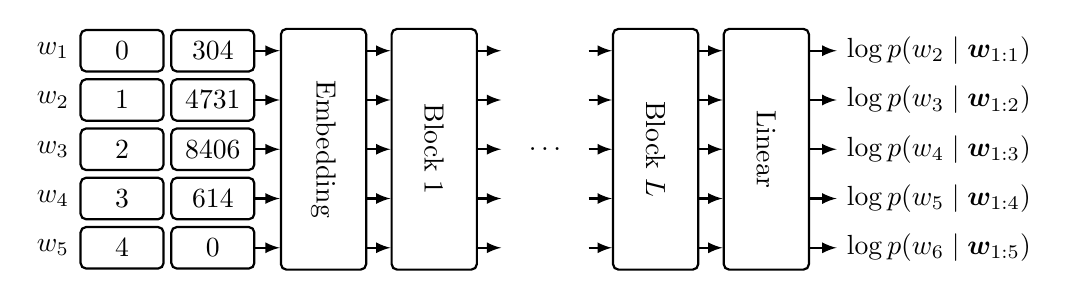
\begin{tikzpicture}[every node/.style={draw, thick, rounded corners=2pt, minimum height=1.5em}, token/.style={minimum width=3em}, vector/.style={minimum width=6em}]
    \node[token] (in1) at (0, 0) {$304$};
    \node[token, below=2pt of in1] (in2) {$4731$};
    \node[token, below=2pt of in2] (in3) {$8406$};
    \node[token, below=2pt of in3] (in4) {$614$};
    \node[token, below=2pt of in4] (in5) {$0$};
    
    \foreach \i [evaluate=\i as \im using {int(\i-1)}] in {1,...,5} {
        \node[token, left=2pt of in\i, label={180:$w_{\i}$}] (pos\i) {$\im$};
    }

    \node[fit=(in1)(in2)(in3)(in4)(in5), inner sep=0pt, xshift=4em, fill=white] (embed_layer) {};
    \node[draw=none, inner sep=0pt, rotate=-90] at (embed_layer.center) {Embedding};
    
    \node[fit=(in1)(in2)(in3)(in4)(in5), inner sep=0pt, xshift=8em, fill=white] (block1) {};
    \node[draw=none, inner sep=0pt, rotate=-90] at (block1.center) {Block 1};
    
    \node[draw=none, fit=(in1)(in2)(in3)(in4)(in5), inner sep=0pt, xshift=12em, fill=white] (block2) {};
    \node[draw=none, inner sep=0pt] at (block2.center) {$\ldots$};
    
    \node[fit=(in1)(in2)(in3)(in4)(in5), inner sep=0pt, xshift=16em, fill=white] (blockL) {};
    \node[draw=none, inner sep=0pt, rotate=-90] at (blockL.center) {Block $L$};
    
    \node[fit=(in1)(in2)(in3)(in4)(in5), inner sep=0pt, xshift=20em, fill=white] (linear) {};
    \node[draw=none, inner sep=0pt, rotate=-90] at (linear.center) {Linear};
    
    \foreach \i [evaluate=\i as \ip using {int(\i+1)}] in {1,...,5} {
        \draw[-latex, thick] (in\i) -- (in\i -| embed_layer.west);
        \draw[-latex, thick] (in\i -| embed_layer.east) -- (in\i -| block1.west);
        \draw[-latex, thick] (in\i -| block1.east) -- (in\i -| block2.west);
        \draw[-latex, thick] (in\i -| block2.east) -- (in\i -| blockL.west);
        \draw[-latex, thick] (in\i -| blockL.east) -- (in\i -| linear.west);
        \node[vector, draw=none, right=21em of in\i] (logproba\i) {$\log p(w_{\ip} \mid \vw_{1:\i})$};
        \draw[-latex, thick] (in\i -| linear.east) -- (logproba\i);
    }
\end{tikzpicture}
\end{minipage}


In this part of the exercise, you will fill in the \texttt{MiniGPT1} class in \texttt{gpt1\_solution\_template.py}. This module contains all the blocks necessary to create this model. In particular, \texttt{self.embedding} is a module responsible for converting sequences of token indices into embeddings (using input and positional embeddings), \texttt{self.layers} is a \href{https://pytorch.org/docs/1.7.1/generated/torch.nn.ModuleList.html}{\texttt{nn.ModuleList}} containing the different \texttt{Block} layers, and \texttt{self.classifier} is a linear layer responsible for classification.

\begin{enumerate}
    \setcounter{enumi}{5}
    \item In the class \texttt{MiniGPT1}, implement the function \texttt{get\_embeddings()} which computes the embedding vectors, based on the input sequences and the positions of the tokens. See the docstrings of \texttt{GPT1Embedding} (in \texttt{utils/embeddings.py}) for details about this module.
    
    \item In the class \texttt{MiniGPT1}, complete the function \texttt{forward()} using the different modules described above. This function must return the log-probabilities (not the logits) of the next words in the sequence.
    
    \item Complete the \texttt{loss()} function, that returns the mean negative log-likelihood of the entire sequences in the mini-batch (and also averaged over the mini-batch dimension). See the definition of the loss in Problem 1.
\end{enumerate}

% You will first implement the \texttt{get\_embeddings()} method which computes the embedding vectors based on the input sequence and the positions of the tokens. You will then implement the \texttt{forward()} method that first calls \texttt{get\_embeddings()} on the input sequence, and then applies all layers sequentially (i.e., the first layer acts on the output of \texttt{get\_embeddings()}, the second layer acts on the output of the first layer, and so on).
% You will then implement the \texttt{loss()} function, which computes the negative log-likelihood loss used to train the mini-GPT. In all cases, please refer to the docstrings of each individual function for a precise description of the intended behavior and the input-output signatures.


\end{homeworkProblem}
\begin{homeworkProblem}
%%%%%%%%%%%%%%%%%%%%%%%%%%%%%%%%%%%%%%%%%
%%%%%%%%%%%%%%%%%%%%%%%%%%%%%%%%%%%%%%%%%
\paragraph{Training language models and model comparison (25pts)}
\vspace{-\baselineskip}

Unlike in classification problems, where the performance metric is typically accuracy, in language modelling, the performance metric is typically based directly on the cross-entropy loss, i.e. the negative log-likelihood ($NLL$) the model assigns to the tokens.
For word-level language modelling it is standard to report \textbf{perplexity (PPL)}, which is the exponentiated average per-token NLL (over all tokens): 
$$\exp\left(\frac{1}{TM}\sum_{t=1}^T \sum_{j=1}^M - \log p(\vw^{(j)}_t \mid \vw^{(j)}_1, ...., \vw^{(j)}_{t-1};\vtheta)\right),$$
where $t$ is the index with the sequence, and $j$ indexes different sequences.
% For Penn Treebank in particular, the test set is treated as a single sequence (i.e. $N=1$).
The purpose of this question is to perform model exploration, which is done using a validation set. As such, we do not require you to run your models on the test set.

You will train each of the following architectures using an optimization technique and scheduler of your choice. For reference, we have provided a \emph{feature-complete} training script (\texttt{run\_exp.py}) that uses the \href{https://pytorch.org/docs/stable/optim.html#torch.optim.AdamW}{\textsc{AdamW}} optimizer. You are free to modify this script as you deem fit. You do not need to submit code for this part of the assignment. However, you are required to create a report that presents the perplexities and training curve comparisions as specified in the following questions.
% either stochastic gradient descent or the ADAM optimizer. The training loop is provided in \textit{run\_exp.py}. 

\textbf{Note}: For each experiment, closely observe the training curves, and report the lowest validation perplexity score across epochs (not necessarily the validation score for the last epoch)

\textbf{Configurations to run}: At the top of the runner file (\texttt{run\_exp.py}), we have provided $12$ experiment configurations for you to run. Together, these configurations span several choices of neural network architecture, optimizer, and weight-decay parameters. Perform the following analysis on the logs.

\begin{enumerate}
    \item[1.] You are asked to run 23 experiments with different architectures, optimizers, and hyperparameters settings. These parameter settings are given to you at the top of the runner file (\texttt{run\_exp.py}). For each of these 23 experiments, plot learning curves (train and validation) of perplexity over both \textbf{epochs} and \textbf{wall-clock-time}. Figures should have labeled axes and a legend and an explanatory caption.
    \item[2.] Make a table of results summarizing the train and validation performance for each experiment, indicating the architecture and optimizer. Sort by architecture, then number of layers, then optimizer, and use the same experiment numbers as in the runner script for easy reference. Bold the best result for each architecture.\footnote{You can also make the table in LaTeX; for convenience you can use tools like \href{https://www.tablesgenerator.com/}{LaTeX table generator} to generate tables online and get the corresponding LaTeX code.} The table should have an explanatory caption, and appropriate column and/or row headers. Any shorthand or symbols in the table should be explained in the caption.
    \item[3.] Which hyperparameters + optimizer would you use if you were most concerned with wall-clock time? With generalization performance?
    \item[4.] Between the experiment configurations 1-4 and 5-8 at the top of \texttt{run\_exp.py}, only the optimizer changed. What difference did you notice about the four optimizers used? What was the impact of weight decay, momentum, and \textsc{Adam}?
    \item[5.] Compare experiments 1 and 5. Which model did you think performed better (LSTM or GPT)? Why?
    \item[6.] In configurations 5-8 and in configurations 11 and 12, you trained a transformer with various hyper-parameter settings. Given the recent high profile transformer based language models, are the results as you expected? Speculate as to why or why not.
    \item[7.] For each of the experiment configurations above, measure the average steady-state GPU memory usage (\texttt{nvidia-smi} is your friend!). Comment about the GPU memory footprints of each model, discussing reasons behind increased or decreased memory consumption where applicable.
    \item[8.] Comment on the overfitting behavior of the various models you trained, under different hyperparameter settings. Did a particular class of models overfit more easily than the others? Can you make an informed guess of the various steps a practitioner can take to prevent overfitting in this case? (You might want to refer to sets of experiments 2, 9, 10 for the LSTM and 6, 11, 12 for GPT -- that evaluate models of increasing capacities).



    %\begin{enumerate}
        % \item What did you expect to see in these experiments, and what actually happens? Why do you think that happens? \vspace{-0.5\baselineskip}
        %\item Referring to the learning curves, qualitatively discuss the differences between the two optimizers in terms of training time, generalization performance, which architecture they're best for, and their relationship to other hyperparameters. \vspace{-0.5\baselineskip}
        %\item Which hyperparameters+optimizer would you use if you were most concerned with wall-clock time? With generalization performance? In each case, what is the ``cost'' of the good performance (e.g. does better wall-clock time to a decent loss mean worse final loss? Does better generalization performance mean longer training time?)\vspace{-0.5\baselineskip}
        % \item Which architecture is most ``reliable'' (decent generalization performance for most hyperparameter+optimizer settings), and which is more unstable across settings? \vspace{-0.5\baselineskip}
        % \item Describe a question you are curious about and what experiment(s) (i.e. what architecture/optimizer/hyperparameters) you would run to investigate that question.\vspace{-0.5\baselineskip}
        % \item % something about how could either of the optimizers be modified to improve their performance? e.g. adding a learning rate schedule to the ``vanilla'' SGD. 
    %    \end{enumerate}
\end{enumerate}

% \item List all of the hyperparameters for each experiment in your report (e.g. specify the command you run in the terminal to launch the job, including the command line arguments). \vspace{-0.5\baselineskip}
% \item Make 2 plots for each optimizer; one which has all of the validation curves for that optimizer over \textbf{epochs} and one over \textbf{wall-clock-time}.\vspace{-0.5\baselineskip}
% \item Make 2 plots for each architecture; one which has all of the validation curves for that architecture over \textbf{epochs} and one over \textbf{wall-clock-time}.\vspace{-0.5\baselineskip}
%\item Make a plot and/or table of any other hyperparamter you vary which you mention in the discussion.


\end{homeworkProblem}



% %\newpage
% \begin{homeworkProblem}
% %%%%%%%%%%%%%%%%%%%%%%%%%%%%%%%%%%%%%%%%%
% %%%%%%%%%%%%%%%%%%%%%%%%%%%%%%%%%%%%%%%%%
% \paragraph{Qualitative examples from trained models  (25pts)}
% \vspace{-\baselineskip}

% For this problem, we will investigate properties of the trained models from Problem 3. Perform the following evaluations for the two models (one LSTM and one GPT) for which the parameters were saved (indicated by the flag --save\_best in the code).

% Run the LSTM and GPT models on the test split of the WikiText-2 dataset and save the generated sentence samples to a text file. Cherrypick 9 samples from the LSTM and 10 samples from the GPT and present them in your report. Discuss whether the generated sequence quality correlates with model validation perplexity. (pick the samples such that 3 of them are ``best'', 3 are ``worst'', and the other 3 are ``interesting'')


% % \begin{enumerate}
% %     % \staritem Compute the average loss at each time-step (i.e. $\mathcal{L}_t$ for each $t$) within validation sequences.  Plot $\mathcal{L}_t$ as a function of $t$, describe the result qualitatively, and provide an explanation for what you observe. Compare the plots for the different architectures.
% %     %
% %     % \item For one minibatch of training data, compute the average gradient of the loss at the \textit{final} time-step with respect to the hidden state at \textit{each} time-step $t$: $\nabla_{\vh_t}\gL_T$.  The norm of these gradients can be used to evaluate the propagation of gradients; a rapidly decreasing norm means that longer-term dependencies have less influence on the training signal, and can indicate \textbf{vanishing gradients}.
% %     % Plot the Euclidian norm of $\nabla_{\vh_t}\gL_T$ as a function of $t$ for the RNN and GRU architectures. Rescale the values of each curve to [0,1] 
% %     % so that you can compare both on one plot. Describe the results qualitatively, and provide an explanation for what you observe, discussing what the plots tell you about the gradient propagation in the different architectures.
% %     % \item 
% %     % Generate samples from the LSTM and GPT models, by recursively making $\hat{\vx}_{t+1} = \argmax P(\vx_{t+1} | \hat{\vx}_1, ...., \hat{\vx}_t)$.\footnote{
% %     % It is possible to generate samples in the same manner from the Transformer, but the implementation is more involved, so you are not required to do so. 
% %     % }
% %     % Make sure to condition on the sampled $\hat{\vx}_t$, \textit{not} the ground truth.
% %     % % Take a random $\hat{\vx}_1$ to start the sequence.
% %     % Produce 20 samples from both the RNN and GRU: 10 sequences of the same length as the training sequences, and 10 sequences of \textit{twice} the length of the training sequences. Do you think that the generated sequence quality correlates with model validation perplexity? Justify your answer. 
    
% %     Choose 3 ``best'', 3 ``worst'', and 3 that are ``interesting''. 
% %     Put all 40 samples in an appendix to your report.
% % \end{enumerate}

% \end{homeworkProblem}

\end{document}